\chapter{Simulations (10 pgs)}

This part of thesis serves as a widen documentation for the \texttt{PyVort} codebase, a new platform to simulate quantum vortex rings. The code is written in well commented Python 3, arranged in a modular structure. The primary aim of this documentation is to highlight which module(s) are involved and how they work.
In appendix, one can find a table of the parameters (user's options) which can be set in the \texttt{config.py} file.

To run the code, there has to be installed only Python 3 (with various libraries) on any OS. All the Python code can be found in the directory \texttt{src/}. The entire project is open-source and can be found as a public \href{https://github.com/KuboBahyl/superfluid}{GitHub} repository. Pull requests of any further development would be definitely appreciated.

At present the code can be run only using infinite boundary conditions. Therefore, only closed-loop vortices can be realized using simulation. However, the codebase flexibly supports the implementation of on-closed loops.

\section{Vortex filament model}

The \texttt{PyVort} code is based on vortex filament (VF) model, a technique pioneerd by Schwarz in the early 1980s. Superfluid vortex filament is represented by a series of mesh points distributed along the centerline of the VF. The motion of the whole VF is summed up by the motion of each mesh point.

\begin{figure}[h]
	\centering
	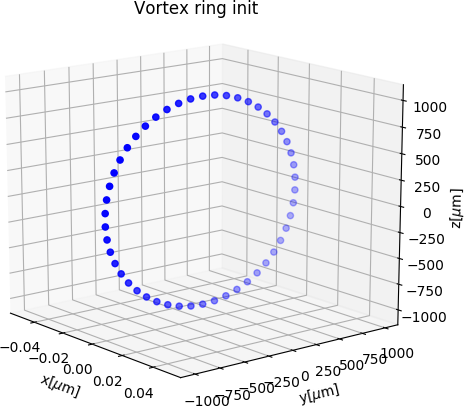
\includegraphics[width=0.5\textwidth]{graphics/simul/ring_init_crop}
	\caption{Example of vortex ring segments}
\end{figure}

More precisely we define the VF as a three dimensional curve
$\vec{s}(\xi, t)$. Here $\xi$ represents arc-lengths and $t$ is time. Each mesh point is given by its coordinates $\vec{s}_i$, direct neighbour indices (previous $(i-1)$ and next mesh point $(i+1)$). This resolves in a directed digraph, which is a good starting point for the initial data structure.

We can construct the tangent vector $\vec{s}^{\prime}$, then normal vector $\vec{s}^{\prime\prime}$, and the binormal vector $\vec{s}^{\prime} \times \vec{s}^{\prime\prime}$ by taking numerical derivatives. Note $\vec{s}^{\prime} = \text{d}\vec{s} / \text{d}\xi$,
and so on.

\subsection*{Finite differences}

Numerical derivatives $\vec{s}^{\prime}$ and $\vec{s}^{\prime\prime}$ need to be properly calculated. At a particular segment with position $\vec{s}_i$ , we define the distance to the particle in-front $\vec{s}_{i+1}$ as $l_{i} = \vert \vec{s}_i - \vec{s}_{i+1} \vert$ and the distance to the particle behind
$\vec{s}_{i-1}$ as $l_{i-1} = \vert \vec{s}_{i-1} - \vec{s}_i \vert$.
By in-front/behind we refer to the particles next/previous along the filament. Similarly, we can define the $l_{i+1}$ and $l_{i-2}$ for the farther particles.

\begin{figure}[h]
	\centering
	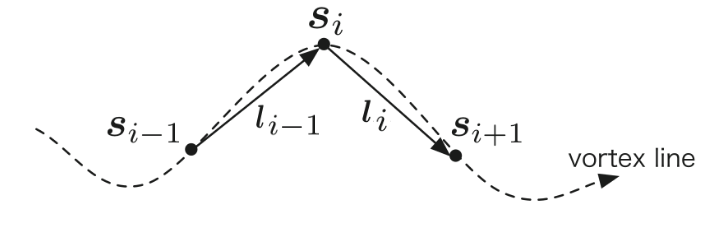
\includegraphics[width=0.8\textwidth]{graphics/simul/finite-diff}
	\caption{Depiction of a few segments and corresponding lengths}
\end{figure}

For accuracy, we approximate all spatial derivatives $\vec{s}_i^{\prime}$, $\vec{s}_i^{\prime\prime}$ by a
fourth-order finite difference method (FD), which can also account the
varying distances along the vortex filament Using FD theorem, we can construct the approximations by taking the Taylor's series expansions. We can then write:

\begin{equation}
\frac{\text{d}^n\vec{s}_i}{\text{d}\xi^n} \approx
A_i\vec{s}_{i-2} +
B_i\vec{s}_{i-1} +
C_i\vec{s}_{i} +
D_i\vec{s}_{i+1} +
E_i\vec{s}_{i+2}
\hspace{1cm}
\text{for} \,n\in\{1,2\}
\end{equation}

Calculation of coefficients $A, B, C, D, E$ can be done in many ways. In code, we use both the analytical solution (closed form) and the solution by inverting the Vandermonde matrix. The first one is obviously faster, but the second one is more reliable.


\subsection*{Biot-Savart discretisation}

We denote the external sources of velocity fields as $\vec{v}_{n,ext}$ and $\vec{v}_{s,ext}$. The equation of motion is then given directly by Schwarz's equation(\ref{schwarz}):

\begin{equation}
\frac{\text{d}\vec{s}}{\text{d}t} =
\vec{v}_{s,ext} + \vec{v}_i + \vec{v}_{\text{mutual}}
\end{equation}

The first difficulty in the VF model come from the calculation of term $\vec{v}_i$. As we shown in (\ref{lia+biot}), this advection term can be split into the LIA part and Biot-Savart integral:

\begin{equation}
\vec{v}_{\text{ind}}^{(i)} =
\frac{\varkappa}{4\pi} (\vec{s}^{\prime} \times \vec{s}^{\prime \prime})
\ln{\Big(\frac{2\sqrt{l_{i-1} l_i}}{a}\Big)}
+ \frac{\varkappa}{4\pi} \int_{\mathcal{L}^{\prime}} \frac{(\vec{r^{\prime}} - \vec{s}) \times \text{d}\vec{r^{\prime}}}{\vert \vec{r^{\prime}} - \vec{s} \vert^3}\,,
\end{equation}

where $l_{i-1}$ and $l_i$ are the arc lengths of the curve between
points $\vec{s}_{i-1}$ and $\vec{s}_i$ and between $\vec{s}_i$ and $\vec{s}_{i+1}$, and $\mathcal{L}^{\prime}$ is the original vortex line without the section between $\vec{s}_{i-1}$ and $\vec{s}_{i+1}$.

Due to our discretisation, the Biot-Savart integral can be rewritten as the sum of line contributions between each $j$ and $j+1$ segments (except for the ones attached to the $i$-th point):

\begin{equation}
\vec{v}_{\text{BIOT}}^{(i)} \approx
\sum_{j \notin \{i-1, i\}}
\frac{\varkappa}{4\pi}
\frac{(R_j + R_{j+1}) (\vec{R}_j \times \vec{R}_{j+1})}{R_j R_{j+1} (R_j R_{j+1} + \vec{R}_j \dotprod \vec{R}_{j+1})}\,,
\end{equation}

where $\vec{R}_j = \vec{s}_j - \vec{s}_i$ and $\vec{R}_{j+1} = \vec{s}_{j+1} - \vec{s}_i$.

\todo comment on time complexity

One way to get around this difficulty is to the updated LIA. In this method we neglect completely the non-local Biot-Savart integral and keep just the local term. This is typically done with a minor adjustments within the log term:

\begin{equation}
\vec{v}_{\text{ind,LIA}}^{(i)} =
\frac{\varkappa}{4\pi} (\vec{s}^{\prime} \times \vec{s}^{\prime \prime})
\ln{\Big(\frac{2R_i}{a}\Big)}\,,
\end{equation}

where $R_i$ is a filament length scale - may be taken as a local curvature of $i-th$ segment. LIA is a very convenient approximation and works very well for calculating the motion of a single vortex ring.

\subsection*{State definition}

In Python 3, the single vortex ring object is represented using \texttt{class} structure. This structure is partially updated after each step, so the \textit{state} of the vortex ring is defined with following properties:

\begin{itemize}
	\item \underline{shape} - a dictionary of three parameters: ring center coordinates $[x_c,y_c,z_c]$, radius $R$ and the direction of desired motion $\{x, y, z\}$ (three possible axis)
	\item \underline{velocity} - the actual velocity of vortex ring center $\vec{v}_c$
	\item \underline{number of segments} - number of segments $N$ the vortex ring is composed of
	\item \underline{segments} - a whole array of particular segments with following attributes:
	\begin{itemize}
		\item \underline{coordinates} - an array of segment coordinates $[x_i,y_i,z_i]$
		\item \underline{previous/next neighbour} - array indices of the \textit{previous} $(i-1)$ and the \textit{next} $(i+1)$ segment from the geometrical point of view
		\item \underline{tangent/curvature} - a tangential and normal vectors $\vec{s}^{\prime}_i$ and $\vec{s}^{\prime\prime}_i$

		\item \underline{LIA velocity} - a self-induced velocity $\vec{v}_{\text{LIA}}(\vec{s}_i)$ driven by the near surrounding.
		\item \underline{BIOT velocity} - a self-induced velocity driven by the farther parts of the vortex ring $\vec{v}_{\text{BIOT}}(\{\vec{s}_j\})$

		\item \underline{Drive velocity} - a velocity given by the mutual friction $\vec{v}_{\text{drive}}(\vec{s}_i)$
		\item \underline{Full velocity} - the sum of external sources $\vec{v}_{s,ext}$, LIA velocity, BIOT velocity and the (quantum) drive velocity
	\end{itemize}
\end{itemize}


\section{Integration}
\begin{itemize}
	\item Euler vs. RK4 step
	\item time stepping
	\item stability
\end{itemize}

\section{Resegmentation}
\begin{itemize}
	\item adding and removing segments
	\item local spline
\end{itemize}

Representative points of vortex lines are added or removed to adjust the spatial
resolution. Typically, when the spacing between s i and s i+1 becomes larger than some
upper limit h max , a new point is added between these two points.

\section{Vortex ring}
\begin{itemize}
	\item initialisation
	\item movement, decreasing radius
	\item comparison with theory
	\item Kelvin waves (?)
\end{itemize}

\section{Future implementations}

If any two lines become very close (a distance less than the separation along the line) then the filaments reconnect, changing the topology of the system.

\newpage
